\documentclass[11pt]{article}

% "review" gives line numbers and page numbers, as in the course reference.
% The \acl@anonymizefalse line below keeps author names visible.
% For a clean copy without line numbers, change "review" to "preprint".
\usepackage[review]{acl}
\makeatletter\acl@anonymizefalse\makeatother

\usepackage{times}
\usepackage{latexsym}
\usepackage[T1]{fontenc}
\usepackage[utf8]{inputenc}
\usepackage{microtype}
\usepackage{inconsolata}
\usepackage{graphicx}
\usepackage{booktabs}
\usepackage{array}
\usepackage{xcolor}
\usepackage{amsmath,amssymb}
\usepackage{enumitem}

% Red, bracketed markers for anything still to be written or measured.
% Search the PDF for "TODO" to find every open item.
\newcommand{\todo}[1]{\textcolor{red}{[TODO: #1]}}

% The teaser figure below the authors needs room, so shrink the default title box.
\setlength\titlebox{3.3cm}

\title{Knowing When Not to Trust Depth:\\
A Learned Per-Pixel Confidence Head for Monocular Depth\\
in Adverse Driving Conditions\\
\large Midterm Report}

\author{Nathan Aday, Alejandro Arteaga, Nathan Bao, Katherine Qiao, Varad Jaideep Tawde}

\begin{document}

\makeatletter
\g@addto@macro\@maketitle{%
  \begin{center}
    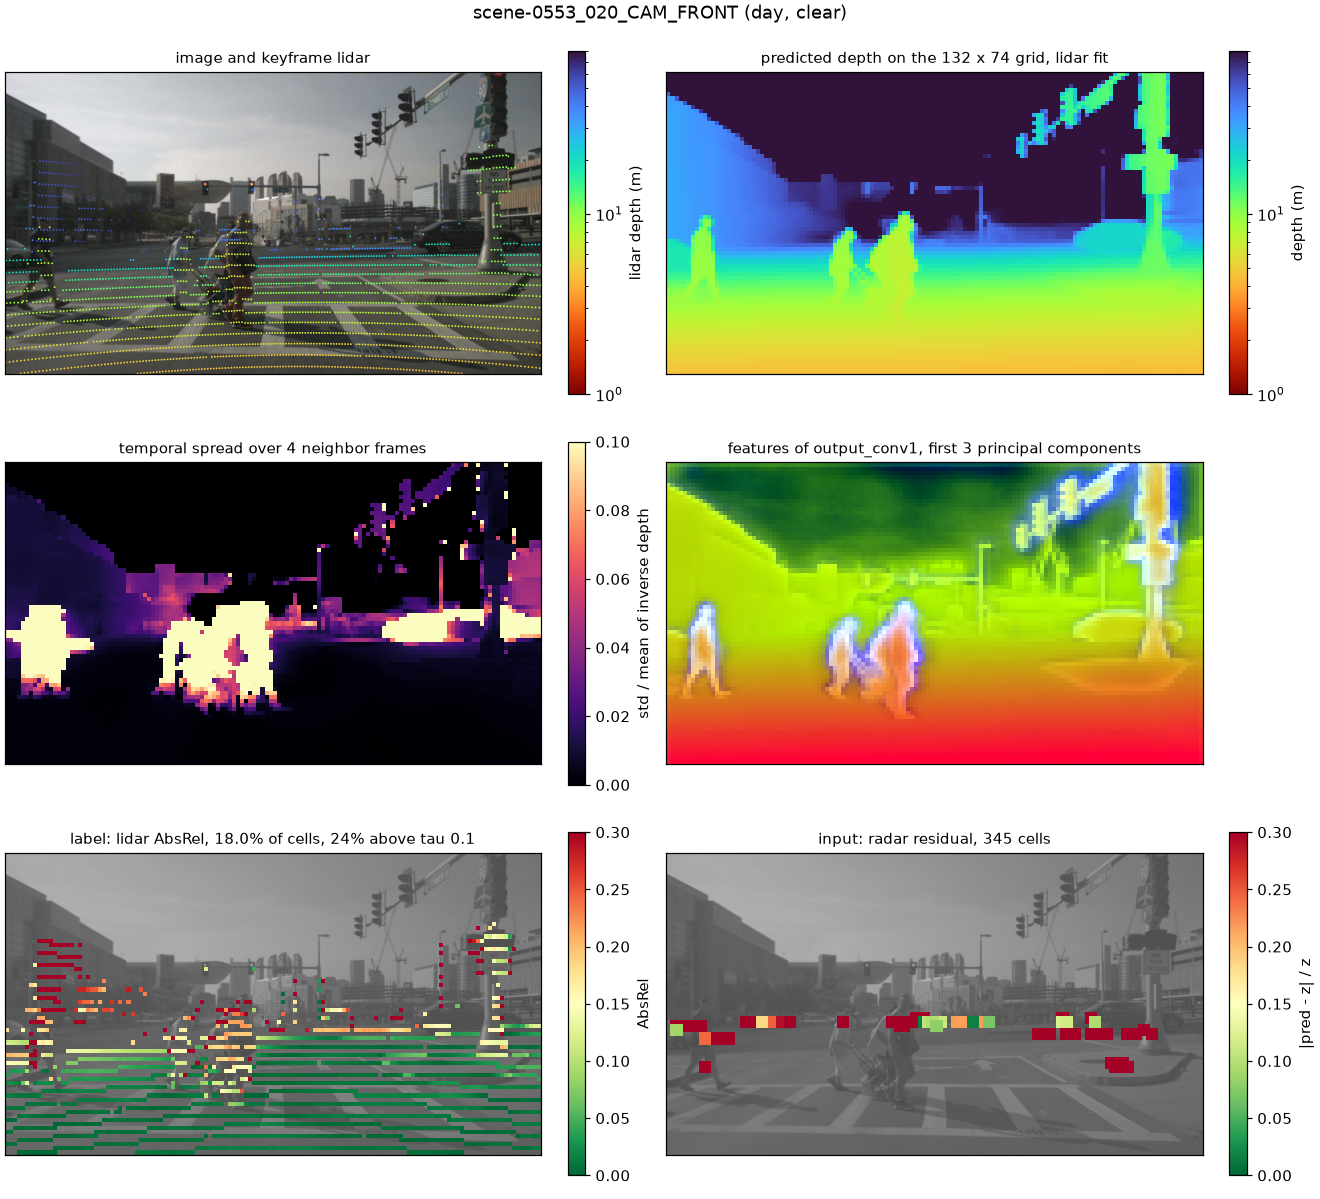
\includegraphics[width=0.46\textwidth]{figures/cache-entry-preview.png}
    \captionof{figure}{One cached training entry (nuScenes scene-0553, CAM\_FRONT, day). Top: the image with projected keyframe lidar, and the Depth Anything V2 prediction after the lidar fit. Middle: the temporal spread input and the first three principal components of the 64 decoder features. Bottom: the lidar AbsRel label on the grid, and the radar residual input. The head reads the four right-hand quantities and must predict the bottom-left map.}
    \label{fig:teaser}
  \end{center}
  \vskip 0.05in}
\makeatother

\maketitle

% ============================================================================
% Owner: all. Rewrite once the Run 1 numbers are in.
% ============================================================================
\begin{abstract}
Monocular depth models such as Depth Anything V2 return a depth value for every pixel and no indication of which values to trust. We are training a small convolutional head that reads the frozen depth model's decoder features, its predicted depth, a temporal-consistency signal, and two radar channels, and outputs per cell the probability that the depth error exceeds a fixed threshold. Labels come from lidar projected into the camera image, so no hand annotation is needed. At the midpoint of the project the full nuScenes dataset is on the USC CARC cluster, a cache of head inputs covers all 204,894 trainval camera images, the head, loss, and training loop are implemented, and the first full training run is in progress. This report reviews the literature the design draws on, describes what is built and where it departs from the proposal, reports the statistics of the cached data and the first training estimate, and sets out the plan for the remaining weeks. \todo{add the Run 1 headline number once evaluated}
\end{abstract}

% ============================================================================
% Owner: Arteaga
% ============================================================================
\section{Introduction}

Depth Anything and similar models supply depth to systems that have no depth sensor. They are used in driving, robotics, augmented reality, and 3D reconstruction, usually as a drop-in component. Every pixel gets a depth value and no measure of reliability: an estimate that is wrong by thirty percent looks exactly like one that is right. The cost of that silence is highest in the conditions where camera depth is least reliable: night, rain on the lens, spray, and low sun. A confidence map lets a downstream consumer weight the depth, discard it, or fall back to another sensor.

This project trains a model to predict that error without touching the depth model. A small convolutional head reads the frozen model's internal features along with its predicted depth, the temporal spread of depth across neighboring frames, a radar residual, and a radar validity mask. It outputs, per grid cell, the probability that the depth there is wrong by more than a threshold. Lidar projected into the image gives the true error at the cells that receive a return, so the head learns from scattered labels and produces a dense map at inference. Lidar is present when the model is built and absent when it runs; radar, which a production car does carry, is present in both.

The rest of the report follows the four components the course asks for. Section~\ref{sec:lit} reviews the literature on depth foundation models, uncertainty for monocular depth, radar-camera fusion, and adverse-condition datasets, and places our design among them. Section~\ref{sec:progress} describes what is implemented and how it departs from the proposal. Section~\ref{sec:results} reports the initial results. Section~\ref{sec:plan} gives the updated plan for the remainder of the term.

% ============================================================================
% Owner: Arteaga
%
% Each \todo{} below is a stub for one reference. Fill them in order; each
% stub should become 2-4 sentences: what the paper does, the one result or
% idea that matters to us, and how it relates to our design. Keep the
% framing sentence at the top of each subsection, or rewrite it once the
% stubs are in. Delete any paper that turns out not to earn its place.
%
% Papers in Docs/Papers/ are named by arXiv id, one PDF per bib entry.
% Every bib entry was checked against arXiv on 2026-11-06.
% ============================================================================
\section{Literature Review}
\label{sec:lit}

\subsection{Monocular depth foundation models}

Our backbone is one of a family of models trained to predict relative depth from a single image across many datasets at once. Three design choices in this family matter for us: the output is affine-invariant disparity rather than metric depth, the decoder is a dense-prediction transformer whose intermediate feature maps are easy to tap, and the model is used frozen by people who cannot retrain it.

\todo{MiDaS \citep{ranftl2020midas}: mixing datasets with a scale-and-shift-invariant loss; why the output needs a per-image fit before it is in meters.}

\todo{DPT \citep{ranftl2021dpt}: the vision-transformer encoder with a convolutional RefineNet-style decoder; name the fusion blocks and the \texttt{output\_conv1} tap we read.}

\todo{Depth Anything \citep{yang2024depthanything}: scaling to 62M unlabeled images with a teacher-student setup; what it changed about robustness.}

\todo{Depth Anything V2 \citep{yang2024depthanythingv2}: synthetic labels plus a large teacher; the ViT-B relative checkpoint we use and the metric fine-tuned variants we chose not to use (see deviation D1).}

\subsection{Uncertainty and confidence for monocular depth}

Most work on uncertainty for depth changes the depth model: it adds a variance output, trains several models, or samples a stochastic one. Our setting forbids that, since the backbone is frozen, so we are closest to the post-hoc methods that read a trained model's behavior without retraining it. This subsection also fixes the evaluation protocol, since sparsification curves and AUSE come from this literature.

\todo{Kendall and Gal \citep{kendall2017uncertainties}: aleatoric versus epistemic uncertainty; heteroscedastic regression with a learned variance. Our head is a classifier on the error, which sidesteps the choice.}

\todo{MC dropout \citep{gal2016dropout}: why it is a baseline in the proposal and why it is dropped (Depth Anything V2 has no dropout, so the passes are identical).}

\todo{Deep ensembles \citep{lakshminarayanan2017ensembles}: the strong but expensive baseline; not applicable to a single frozen checkpoint.}

\todo{Ilg et al. \citep{ilg2018uncertainty}: the origin of the sparsification plot and the area between the model's curve and the oracle, which Poggi et al. adopt as AUSE.}

\todo{Poggi et al. \citep{poggi2020uncertainty}: the systematic comparison for monocular depth; define AUSE and AURG as we report them; the flip-augmentation ``Post'' baseline we adopt and the ``Self'' learned-confidence head that is the closest relative of ours.}

\todo{Hornauer and Belagiannis \citep{hornauer2022gradient}: post-hoc uncertainty from gradients on a frozen depth model; the nearest prior work to a head that leaves the backbone untouched.}

\subsection{Radar-camera fusion for depth and occupancy}

Radar is the sensor a production car has in rain and at night when the camera degrades, and recent work fuses it with images to improve depth or 3D perception. We use it differently: the radar channels tell the head where the frozen depth disagrees with an independent range measurement, so the output is a confidence map rather than a better depth map.

\todo{Lin, Dai, and Van Gool \citep{lin2020radardepth}: dense depth from an image plus sparse nuScenes radar; what they report about radar noise and the lack of elevation, which we see as a radar residual about five times the lidar error.}

\todo{HyDRa \citep{wolters2025hydra}: fuses radar features with image features in the perspective view before the depth head (Height Association Transformer) and in BEV (Radar-weighted Depth Consistency); state of the art on nuScenes detection and Occ3D. Contrast: they change the depth, we score it.}

\todo{LiCROcc \citep{ma2024licrocc}: distills lidar-camera occupancy knowledge into radar and radar-camera students (CMRD, BRD, PDD modules); the teacher-student view of lidar as training-time-only supervision is the same stance our labels take.}

\todo{BEVCar \citep{schramm2024bevcar}: camera-radar BEV segmentation; the source of the day/rain/night split of the nuScenes val scenes (111/24/15 scenes) that all our per-condition numbers will use.}

\todo{Occ3D \citep{tian2023occ3d}: the occupancy benchmark for the stretch goal; what mIoU measures there.}

\subsection{Adverse-condition driving datasets}

The method needs lidar, camera sequences, calibrated radar, and condition labels in the same recording. The datasets below are the candidates we reviewed; nuScenes is the one in use.

\todo{nuScenes \citep{caesar2020nuscenes}: 1,000 scenes, 6 cameras, 32-beam lidar, 5 radars, Boston and Singapore, day/night/rain; the official 700/150/150 split; what the radar does and does not provide (no elevation, sparse).}

\todo{md4all \citep{gasperini2023md4all}: monocular depth under night and rain on nuScenes; the per-condition val counts (4,449 day-clear, 1,088 rain, 602 night keyframes) and the fact that the test split carries no weather metadata.}

\todo{STF / DENSE \citep{bijelic2020seeing}: fog, snow, and rain with a fog chamber where visibility is controlled; the stage-2 candidate for weather nuScenes lacks; access is by request.}

\todo{Zenseact Open Dataset \citep{alibeigi2023zod}: Nordic weather, three lidars, permissive license; radar added in the 2025 release, which makes it usable if the radar ablation shows the channel matters.}

\subsection{Where this work sits}

\todo{Rewrite once the stubs above are filled.} Two contrasts define the project. First, the fusion literature uses radar to improve the depth itself; we use it to predict where the depth is wrong and leave the depth model untouched. Second, the uncertainty literature mostly retrains or samples the depth model; we train only a small head on top of a frozen one, which is the situation of everyone who uses a public depth checkpoint. Whether the frozen decoder features carry enough information to predict the model's own error, and how much radar and temporal consistency add, are the questions the experiments answer.

% ============================================================================
% Owner: Aday and Bao (method, data, infrastructure). Arteaga: deviations table.
% Drafted from Docs/worklog.md, Docs/Wiki/*.md, Docs/proposal-vs-pipeline.md.
% ============================================================================
\section{Progress So Far}
\label{sec:progress}

\subsection{Method as implemented}

\paragraph{Backbone.} The stock relative Depth Anything V2 ViT-B checkpoint \citep{yang2024depthanythingv2}, frozen, run once per image at $924 \times 518$. Its output is disparity with unknown scale and shift, so each cached entry carries two per-image least-squares fits of disparity to inverse depth: one against the keyframe lidar, used for the labels and the temporal channel, and one against the radar points, used for the radar residual.

\paragraph{Inputs.} Everything lives on a $264 \times 148$ grid, the ViT patch grid times four, where one cell covers about $6 \times 6$ pixels. The head input has 68 channels (Table~\ref{tab:inputs}), each standardized by its training-set mean and standard deviation. Channel groups can be switched off at load time for ablations.

\begin{table}[t]
  \centering
  \small
  \setlength{\tabcolsep}{4pt}
  \begin{tabular}{@{}l l p{3.2cm}@{}}
    \toprule
    \textbf{Ch.} & \textbf{Input} & \textbf{How it is made} \\
    \midrule
    0--63 & Decoder features & \texttt{output\_conv1} tap, 64 channels, area-averaged to the grid \\
    64 & Depth & Disparity divided by its image mean; no fit \\
    65 & Temporal spread & Std over mean of inverse depth across frames at $\pm1, \pm2$ (12\,Hz), ego-motion compensated \\
    66 & Radar residual & $|\hat d - z| / z$ under the radar fit, 5 sweeps, radius 1 cell \\
    67 & Radar validity & 1 where the residual holds a measurement \\
    \bottomrule
  \end{tabular}
  \caption{The 68 input channels of the confidence head.}
  \label{tab:inputs}
\end{table}

\paragraph{Labels.} For each lidar return within 1--80\,m, the absolute relative error (AbsRel) of the fitted prediction at that pixel is placed in its grid cell; the nearest point wins a cell. The target is $\mathbb{1}[\mathrm{AbsRel} > \tau]$ with $\tau = 0.10$, and a mask marks the labeled cells. About 9\% of cells on the $264 \times 148$ grid carry a label, about 3,600 per image, which corresponds to 0.25\% of pixels, in line with the proposal's ``under one percent''.

\paragraph{Head and loss.} Three $3 \times 3$ convolutions with ReLU and widths 64, 64, 32, then a $1 \times 1$ convolution to one logit per cell. The loss is binary cross-entropy over labeled cells only, with positives weighted by the negative-to-positive ratio.

\paragraph{Training.} AdamW, learning rate $10^{-3}$, weight decay $10^{-4}$, cosine schedule, batch size 8, 8 epochs. The dev split is 10\% of the training scenes, capped at 3,000 images. The checkpoint kept is the one with the lowest dev loss (deviation D14).

\subsection{Data and infrastructure}

Full nuScenes v1.0 (trainval and test, over 800\,GB) was downloaded to the USC CARC cluster on 2026-10-19 with a resumable, MD5-checked script adapted from an open-source downloader. The cache of head inputs for all 204,894 trainval camera images was built as a 16-shard GPU job array and verified twice. Each entry is one \texttt{.npz} plus one \texttt{.json}: the fp16 feature map, the disparity grid, the temporal spread and its frame count, the lidar and radar points with the model disparity at each, and the two fits. Labels and radar channels are computed when an entry loads, so $\tau$, the radar radius, and the choice of fit are settings rather than rebuilds. A fingerprint of the content settings lets a stopped build resume. A backup copy is on Hugging Face (\texttt{nadayusc/confhead-cache}). \todo{confirm the upload completed and a download restores the cache.}

Training runs as a single-GPU (A100 or A40) batch job with a 12-hour limit and resumes from the last checkpoint. The evaluation code holds a first version of sparsification curves, AUSE, AURG, rejection AUC, and ECE, with synthetic tests for the curves; data loading from the cache and bootstrap confidence intervals are still to be written. Three notebooks document the cache, training, and evaluation workflows.

\subsection{Deviations from the proposal}

Table~\ref{tab:deviations} lists where the implementation departs from the pre-proposal and the internal Run~1 plan. Three items from the proposal are not built yet and each has a planned action (Section~\ref{sec:plan}): the flip-augmentation baseline, the BEVCar weather split, and the frame selector. Three others are accepted as deviations with a reason. MC dropout is dropped because every dropout rate in the Depth Anything V2 encoder is zero and the decoder has none, so repeated passes are identical; flip disagreement covers its role. Predictions are on the $264 \times 148$ grid rather than at image resolution; every method is scored on the same labeled cells, so the grid costs each one equally. The label share is about 9\% of cells rather than ``under 1\% of pixels''; both are true, since nearly every lidar point gets its own cell.

\begin{table*}[t]
  \centering
  \small
  \setlength{\tabcolsep}{4pt}
  \newcolumntype{P}[1]{>{\raggedright\arraybackslash}p{#1}}
  \begin{tabular}{@{}l P{2.2cm} P{5.1cm} P{5.1cm} P{1.9cm}@{}}
    \toprule
    \textbf{ID} & \textbf{Subject} & \textbf{Proposal / Run 1 plan} & \textbf{Implemented} & \textbf{Status} \\
    \midrule
    D1 & Depth model & Metric checkpoint (vkitti), in meters, no fit & Relative ViT-B with per-image lidar and radar fits & Decided; lidar leakage noted \\
    D2 & Feature storage & Run the model inside the training loop (no store) & Features cached on a coarser grid, 5.4\,MB/image & Follows pre-proposal \\
    D3 & Feature map & \texttt{path\_1}, 128 ch.\ at $296 \times 528$ & \texttt{output\_conv1}, 64 ch.\ at $264 \times 148$ & Within Form B \\
    D4 & Temporal channel & Deferred to Run 2 & Built: relative std of inverse depth, 4 extra passes & Follows Form B \\
    D5 & Depth channel & $D/80$ in meters & Disparity over its image mean & Follows from D1 \\
    D6 & Radar residual & Clipped to $[0,1]$, radius 2, keyframe sweep & Unclipped, radius 1, 5 sweeps, radar fit; empty when the fit fails (13.5\% of mini) & Ablation planned \\
    D7 & Label placement & Bilinear sample at each lidar pixel & Nearest point wins a grid cell & Decided \\
    D8 & CAM\_BACK ego body & Drop lidar hidden by the trunk (3.2\% of CAM\_BACK) & Not masked & Open \\
    D9 & Occlusion bleed-through & Not covered & Not removed (0.35\% of lidar pixels) & Open \\
    D10 & Data & Full nuScenes with train/dev/report splits & Done: trainval cache built on CARC & Resolved \\
    D11 & Weather tag & Decide how to count ``night, after rain'' & Substring rule: such a scene is night and rain & Open; BEVCar split planned \\
    D12 & Label gate & Positive rate within 5--70\% on train & 37.6\% positive on trainval & Inside gate \\
    D13 & Images with no fit & Not covered & 4 night images have no lidar fit, so no labels & Open \\
    D14 & Checkpoint choice & Lowest dev AUSE & Lowest dev loss; AUSE computed afterwards & Decided \\
    \bottomrule
  \end{tabular}
  \caption{Deviations between the plans and the implementation. ``Open'' items are listed with their resolution in Section~\ref{sec:plan}.}
  \label{tab:deviations}
\end{table*}

% ============================================================================
% Owner: Tawde and Qiao (evaluation), with Aday and Bao for the Run 1 numbers.
% Drafted from confhead/results/*.md, Docs/worklog.md, and the Run 1 log.
% ============================================================================
\section{Initial Results}
\label{sec:results}

No AUSE or AURG has been measured on the full data yet; Run~1 is training at the time of writing. This section reports what the cached data says about the task and the measured training estimate, and leaves the result table and figures as placeholders to be filled when Run~1 finishes.

\subsection{Cache and label statistics}

Table~\ref{tab:cachestats} summarizes the development cache built on nuScenes v1.0-mini at a $132 \times 74$ grid and the counts measured on the full trainval cache. Three observations shape the experiments. First, the task is learnable in principle: labels cover a quarter of the coarse-grid cells, and 37\% of labeled cells are positive at $\tau = 0.10$, inside the 5--70\% gate the Run~1 plan set. Second, night is harder: the median per-image AbsRel is 0.052 by day and 0.079 at night, and the only images with no usable lidar fit are four night frames. Third, the radar residual is noisy: its median is 0.25 under the radar fit and 0.28 under the lidar fit, about five times the lidar-measured depth error, and 13.5\% of mini images have no radar fit at all. The likely cause is that nuScenes radar has no elevation, so a radar point can project onto a pixel showing another surface. Whether the channel still helps is the subject of the planned radar ablation.

\begin{table}[t]
  \centering
  \small
  \setlength{\tabcolsep}{4pt}
  \begin{tabular}{@{}l r r@{}}
    \toprule
    & \textbf{mini ($\times 2$)} & \textbf{trainval ($\times 4$)} \\
    \midrule
    Camera images & 2,424 & 204,894 \\
    Cache size & 3.43\,GB & \todo{TB} \\
    Build time & 42\,min & \todo{h} \\
    Lidar points / image & 3,613 & \todo{} \\
    Radar points / image (5 sweeps) & 150 & \todo{} \\
    Images with a lidar fit & 99.8\% & \todo{} \\
    Images with a radar fit & 86.5\% & \todo{} \\
    Labeled cells & 26.2\% & 25.1\%$^{\dagger}$ \\
    Positive labels ($\tau = 0.10$) & 37.2\% & 37.6\% \\
    Median AbsRel, day / night & 0.052 / 0.079 & \todo{} \\
    Median radar residual & 0.25 & \todo{} \\
    \bottomrule
  \end{tabular}
  \caption{Statistics of the cached head inputs and labels. $^{\dagger}$Measured on the training split at the $\times 4$ grid by the Run~1 estimate. \todo{fill the trainval column from the cache summary on CARC.}}
  \label{tab:cachestats}
\end{table}

Two label pitfalls were measured on mini and are open items (D8, D9): 3.2\% of CAM\_BACK lidar pixels fall on the ego vehicle's trunk, and about 0.35\% of lidar pixels are returns from behind a nearer object that bleed through. Both place labels on surfaces the camera does not see.

\subsection{Run 1: first full training run}

The Run~1 estimate on the trainval cache (2026-10-28) uses 631 training scenes (110,929 images, including 76 night and 125 rain scenes) and 69 dev scenes (3,000 of 12,150 images). Of the training cells, 25.1\% carry a label and 37.6\% of those are positive, giving a class weight of 1.658. The cache loads at 28 images/s while a training step runs at 1,007 images/s, so data loading sets the pace: one epoch takes about 66 minutes and 8 epochs about 8.8 hours, inside the 12-hour job limit. The run started on 2026-10-28.

\todo{Per-epoch train and dev loss, and dev AUSE per epoch, once the job ends.} On mini, the two checkpoint rules disagreed: dev AUSE was lowest after epoch 1 while dev loss was lowest after epoch 8, which is why D14 computes AUSE on the loss-selected checkpoint and reports both curves.

\begin{figure}[t]
  \centering
  \fbox{\parbox{0.9\columnwidth}{\centering\vspace{2.5cm}\todo{Run 1 loss curve: train and dev masked BCE per epoch, with dev AUSE on a second axis}\vspace{2.5cm}}}
  \caption{Run 1 training curves. \todo{replace with the figure from the run folder.}}
  \label{fig:losscurve}
\end{figure}

\subsection{Sparsification results (pending)}

Table~\ref{tab:results} and Figure~\ref{fig:sparsification} are the primary deliverable and will be filled from the Run~1 checkpoint. Every method is scored on the same labeled cells of the nuScenes val split, overall and per BEVCar condition group.

\begin{table*}[t]
  \centering
  \small
  \setlength{\tabcolsep}{3pt}
  \begin{tabular}{@{}l cc cc cc cc@{}}
    \toprule
    & \multicolumn{2}{c}{\textbf{All}} & \multicolumn{2}{c}{\textbf{Day}} & \multicolumn{2}{c}{\textbf{Night}} & \multicolumn{2}{c}{\textbf{Rain}} \\
    \cmidrule(lr){2-3}\cmidrule(lr){4-5}\cmidrule(lr){6-7}\cmidrule(lr){8-9}
    \textbf{Method} & AUSE & AURG & AUSE & AURG & AUSE & AURG & AUSE & AURG \\
    \midrule
    Random removal & -- & 0 & -- & 0 & -- & 0 & -- & 0 \\
    Temporal spread & \todo{} & \todo{} & \todo{} & \todo{} & \todo{} & \todo{} & \todo{} & \todo{} \\
    Flip disagreement & \todo{} & \todo{} & \todo{} & \todo{} & \todo{} & \todo{} & \todo{} & \todo{} \\
    Head (ours) & \todo{} & \todo{} & \todo{} & \todo{} & \todo{} & \todo{} & \todo{} & \todo{} \\
    Head, no radar & \todo{} & \todo{} & \todo{} & \todo{} & \todo{} & \todo{} & \todo{} & \todo{} \\
    Oracle & 0 & -- & 0 & -- & 0 & -- & 0 & -- \\
    \bottomrule
  \end{tabular}
  \caption{AUSE (lower is better) and AURG (higher is better) on the nuScenes val split, per BEVCar condition group. \todo{fill from Run 1; add scene counts per group.}}
  \label{tab:results}
\end{table*}

\begin{figure}[t]
  \centering
  \fbox{\parbox{0.9\columnwidth}{\centering\vspace{2.5cm}\todo{Sparsification curves: AbsRel of the remaining cells against the fraction removed, for the head, temporal spread, flip disagreement, random removal, and the oracle; one panel per condition}\vspace{2.5cm}}}
  \caption{Sparsification curves. \todo{replace with the evaluation output.}}
  \label{fig:sparsification}
\end{figure}

% ============================================================================
% Owner: Arteaga, with each item's owner named. Drafted from
% Docs/training-next-actions.md, Docs/worklog.md, and the dataset strategy.
% ============================================================================
\section{Updated Plan}
\label{sec:plan}

\subsection{Remaining work}

Each item names its owner and what ``done'' means. None of the items needs a rebuild of the cache: the flip baseline writes a side file, and the BEVCar split, the radar variants, and the frame selector all work from arrays every entry already holds.

\begin{enumerate}[leftmargin=*, itemsep=2pt]
  \item \textbf{Finish and evaluate Run 1} (Aday, Bao; Tawde, Qiao). Check the per-epoch dev loss, save the loss curve and dev AUSE with the checkpoint, write a $p_\mathrm{error}$ map for every val image, and report AUSE and AURG for the head, random removal, and the oracle. Done when Table~\ref{tab:results} has its first three rows.
  \item \textbf{Flip-augmentation baseline} (Aday, Bao). Run the backbone on the horizontally flipped val keyframes (about 36,000 images), align with a lidar-free scale-and-shift fit, and score the per-cell relative difference. Done when its AUSE and AURG are in the table.
  \item \textbf{BEVCar weather split} (Tawde, Qiao). Adopt the 111 day, 24 rain, and 15 night val scenes (4,449, 968, and 602 keyframes) from BEVCar's released lists, report every number per group with its scene count, compare the cache's keyword tags against the lists, and add a label-count table per group. Done when the per-group columns of Table~\ref{tab:results} are filled.
  \item \textbf{Radar ablation} (Aday, Bao). Train and score the head with radar off, with the radar fit, and with the lidar fit; try a trimmed radar fit; report the radar residual next to the lidar AbsRel. Done when the report says whether the radar channel helps.
  \item \textbf{Temporal ablation and features-only head} (Aday, Bao). Score the raw temporal spread as a baseline and the head on decoder features alone. These decide what stays in the model.
  \item \textbf{Complete the evaluation code} (Tawde, Qiao). Cache data loading, bootstrap confidence intervals, and the sparsification figure. \todo{date}
  \item \textbf{Frame selector} (Tawde, Qiao). Rank whole images by mean $p_\mathrm{error}$ and by mean raw temporal spread, drop the worst $N$\%, and draw both on the same image-level sparsification axes. This is the first downstream consumer.
  \item \textbf{Resolve the open deviations} (all). D8: mask the CAM\_BACK ego body by a fixed image region. D9: decide whether to drop bleed-through points from the labels. D11: adopt the BEVCar rule for rainy night scenes. D13: drop the no-fit images or label every cell as wrong, and say which. \todo{record each decision}
  \item \textbf{Second dataset} (Arteaga). Request STF / DENSE access; if the radar ablation shows the radar channel is not carrying the head, evaluate on ZOD instead.
  \item \textbf{Final report and repository} (all). Results per condition, the deviations table with every item closed, the model card on Hugging Face, and the reproducibility notebooks.
\end{enumerate}

\subsection{Timeline}

\begin{table}[h]
  \centering
  \small
  \setlength{\tabcolsep}{4pt}
  \begin{tabular}{@{}l p{4.6cm}@{}}
    \toprule
    \textbf{Week of} & \textbf{Milestone} \\
    \midrule
    Nov 16 & Run 1 evaluated; flip baseline scored; BEVCar split adopted (items 1--3) \\
    Nov 23 & Radar and temporal ablations trained and scored (items 4--5); evaluation code complete (item 6) \\
    Nov 30 & Frame selector; open deviations closed; Run 2 if an ablation changes the input set (items 7--8) \\
    Dec 7 & Final figures and tables; report writing; repository cleanup (items 9--10) \\
    \todo{final due date} & Final report and presentation \\
    \bottomrule
  \end{tabular}
  \caption{Plan for the remainder of the term. \todo{confirm the final report deadline and adjust.}}
  \label{tab:timeline}
\end{table}

The stretch goal from the proposal, weighting the camera-to-voxel lift of an occupancy network by the confidence map and measuring mIoU on Occ3D, stays conditional: it starts only if items 1--5 are done by the week of November 30.

\subsection{Risks}

Training is bound by cache loading at 28 images/s, so each additional training run costs about nine GPU-hours; the ablations are budgeted as four such runs. The radar residual is about five times noisier than the lidar error, so the radar channels may add nothing, which is a reportable negative result rather than a failure. The label gate and all error statistics are measured with the relative model and a lidar fit, so the report must state that the fit uses a sensor the deployed system lacks. The Hugging Face backup of the cache has not yet been verified by a restore.

\bibliography{references}

\end{document}
